\documentclass[../main.tex]{subfiles}
\begin{document}
\chapter{Design}
\section{System Overview}
\begin{figure}[h!]
\centering
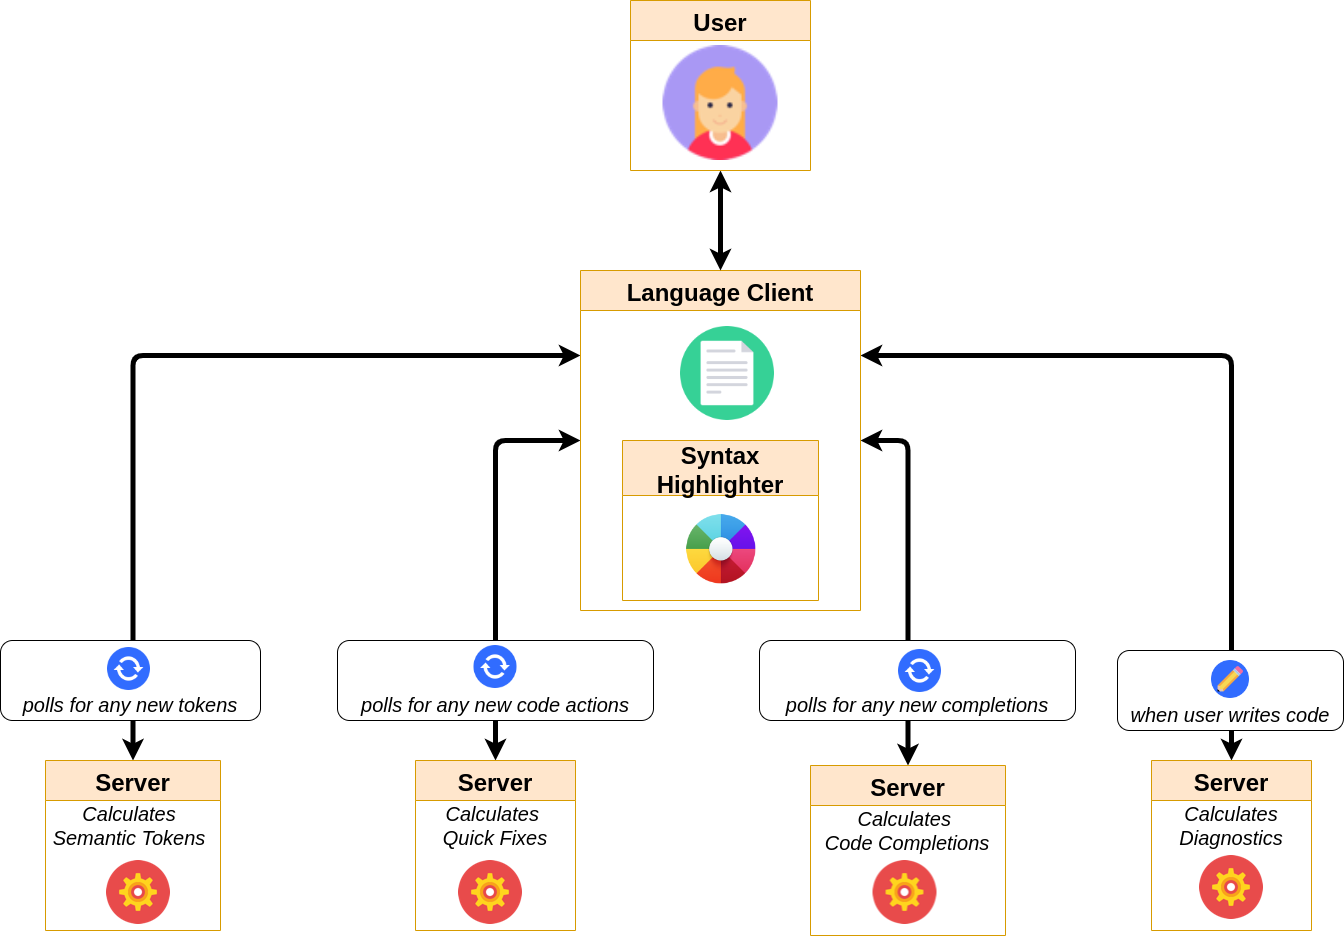
\includegraphics[width = \linewidth]{./figures/le-editor.png}
\caption{A diagram showing the overall structure of the Logical English editor.}
\label{fig:system-overview}
\end{figure}
\todo[inline]{Increase the font size.}
% The Logical English editor is a complex system with multiple components. Before I go into detail describing how the editor was designed, I believe it will be helpful to supply some context by giving an overview of the editor's components and how they relate to each other.
The overall structure of the editor is described in Figure \cite{fig:system-overview}. The user interacts with the editor through the language client. The language client takes on the rules of the syntax highlighter to highlight basic syntactic features of the user's document. The language client highlights semantic features of the document, along with presenting any code completions or quick fixes, by routinely polling the language server for this data. The language server presents error diagnostics by requesting diagnostic data from the server whenever the user makes a change to the document.

\section{Requirements Approach}
\subsection{Why a Language Server?}
When deciding what type of language extension to create, we surveyed a variety of options. 
\\
\\
Logical English is currently edited on the SWISH platform. This runs on Codemirror, a JavaScript framework for creating web-based code editors. This meant that writing the language server entirely in Codemirror was the initial choice.
\\
\\
However, at the time, the SWISH platform was written in Codemirror 5, but the maintainers were considering migrating to Codemirror 6. Prematurely writing the language extension in Codemirror 6 would be too much of a risk, as migration was uncertain, and users would not be able to test the extension until it was migrated. However, developing the extension in Codemirror 5 was also sub-optimal. This was because migration to Codemirror 6 would involve a number of breaking changes \cite{codemirror_migration}, for example, changes that would have entirely restructured interacting with Logical English documents.
\\ 
\\ 
This prompted us to then consider Monaco. \todo[inline]{Why were we considering Monaco? How would Monaco have worked with SWISH?}.
\\ 
\\ 
After researching other options, I found that an editor-agnostic language server would leave us open to using a variety of editors. Using the Language Server Protocol, a single language server would be able to connect to any language client that supports the protocol. This includes language clients written in online editors such as Codemirror 6 \cite{codemirror_6_language_server} and Monaco \cite{monaco_language_server}, along with some of the most popular desktop code editors, such as Visual Studio Code \cite{vsc_langserver_docs}, Visual Studio \cite{visual_studio_language_server} and IntelliJ \cite{intellij_language_server} \cite{ide_rankings}. 
\\
\\
I was hoping that Codemirror 5 would support the Language Server Protocol, so that I could immediately publish the editor to the SWISH platform. Unfortunately, the Codemirror 5 development team are not willing to integrate with the protocol \cite{codemirror5_no_lsp}. 
\\
\\
Looking elsewhere, I found an unmaintained, alpha release of a Codemirror 5 plugin that claimed to be able to communicate with language servers using the Language Server Protocol \cite{lsp_editor_adapter}. To test this, I created a simple language server, extending the sample language server created by Microsoft \cite{lsp_sample_server} with basic code completion and code action features. The sample server came with a language client, which displayed the three kinds of features as expected. However, after connected the language server to the Codemirror 5 plugin according to the plugin's instructions, the Codemirror 5 language client was only able to display the error diagnosis feature. Although I cannot be sure of why the Codemirror 5 client failed to display all three of the features, after inspecting the TCP packets with Ubuntu Linux's built-in \codeword{netcat} command, the cause appeared that the Codemirror 5 plugin was using a different encoding for its requests than the encoding that the language server used.
\\
\\
This lead my supervisors and I to have to decide between a Codemirror 5 extension, that would be usable immediately but may soon become outdated, versus a language server that would need to be used through a new editor, but could be used through many different editors, online or desktop. I advocated for the latter option and my supervisors agreed. Logical English is still in an early stage of development and adoption, so producing a language server would give the flexibility needed to branch out to all kinds of coding environments.

\subsection{Why a Visual Studio Code client?}
Although a language server could be connected to many different language clients, to keep the scope of the project manageable I focused on developing one language client. I had two requirements when searching for the right client for the language server: I was looking to maximise both the amount of features that the client supported, and the popularity of the language client. 
\\
\\
Surprisingly, the latter criterion proved to be a lot easier to judge than the former. Stack Overflow, one of the most popular websites for the programming community, conducts global surveys every year monitoring the programming community's trends. In 2021, out of over 80,000 responses, Visual Studio Code had ``a significant lead as the Integrated Development Environment (IDE) of choice across all developers", with over 70\% of responders using the IDE  \cite{ide_rankings}. This made Visual Studio Code a clear choice in terms of popularity. 
\\
\\
However, I also considered two runner-up IDEs in the survey, Visual Studio and IntelliJ, with 29\% and 33\% of responders using the IDEs. As mentioned in the previous section, all three IDEs support language servers. However, unlike Visual Studio Code, Visual Studio and IntelliJ are quite complex, heavyweight IDEs, with a larger application size, longer install time, and complex user interface. A large part of the target audience of Logical English are logicians and lawyers, neither of which are as a group that involves itself with enterprise programming. This lead me to decide that the simpler the IDE, the better; having to use an enterprise-programming IDE would be inconvenient and off-putting. 
\todo[inline]{Investigate how well Visual Studio Code is suited for people not used to programming}
\\
\\
Visual Studio Code has strong support for using language servers following the Language Server protocol. Although I could only truly verify this after having built a language server with a Visual Studio Code client, there were many indications of this that were available during my initial research. Microsoft's extensive documentation of the features available with a Visual Studio Code client, \cite{vsc_langserver_features}, along with the wide list of language servers built for Visual Studio Code \cite{open_source_language_servers} lead me to trust Visual Studio Code as a language client that was technically capable to the task. 
\todo[inline]{Pick a language server from the list and explain how it has all the required features.}


\subsection{Why a separate Syntax Highlighter?}
Although language servers can mark code for highlighting (and, indeed, mine does), it is common to delegate the majority of the highlighting to the client. This is done for efficiency reasons. It is often the case that some highlighting features can be described by applying simple search patterns to the document: rules such as `\codeword{if} is a keyword' or `text of the form \codeword{*a _*} is a template argument'. These rules are computationally simple, so they do not need to be computed by the language server. In fact, doing so would incur delay in waiting for the server to receive the request to highlight the document, and respond with the highlighting data. For this reason, the client applies these search patterns itself. This is done by specifying these search patterns in a document, referred to as the `syntax highlighter' or `language grammar', which the language client reads at it launches.
\\
\\
A Visual Studio Code requires a syntax highlighter written in a JSON document according to the TextMate grammar \cite{textmate_grammars_spec}. This is standard amongst language clients, with Codemirror 6, Visual Studio and IntelliJ also supporting syntax highlighting using TextMate grammar \cite{codemirror_textmate}, \cite{visual_studio_textmate}, \cite{intellij_textmate}.
%
%
%
\section{Development Technology}
\subsection{Language Server}
Before any work could be done, I needed to decide on which technology to use. This was dictated mainly by the programming language involved. The following features were needed:
\\
\\
\textbf{Linux, Windows and Mac OS support} \\
The language server had to be able to connect to offline editors, and therefore run on user's desktops. This meant that the latest editions of the three most popular operating systems -- Linux, Windows and Mac OS X -- had to be supported.
\\
\\
\textbf{Support for strong typing} \\
Since creating a language server is a large and complex project, I required a strongly-typed programming language. This was both in order to both avoid mistakes that could be detected before run-time, and to receive context-aware support from my IDE.
\\
\\
\textbf{A Language Server Protocol API} \\
Writing Language Server Protocol requests manually would be inefficient, time-consuming and a potential cause of errors. A library that abstracted away the exact layout and content of Language Server Protocol requests would aid productivity.
\\ 
\\
These last two requirements only left two libraries: the \\ 
\texttt{Microsoft.VisualStudio.LanguageServer}, written for C\# \cite{visual_studio_language_server}, and \\ 
\texttt{vscode-languageserver}, written for TypeScript \cite{vsc_langserver_docs}. Since these language server libraries were both created by Microsoft \footnote{This is because Microsoft also created the Language Server Protocol.}, they are both structured quite similarly. 
\\
\\
In the end, the TypeScript library was chosen over the C\# library. Both libraries being quite similar, this decision was made because TypeScript was better suited for the task than C\#. The Language Server Protocol communicates using JSON, and it is easier to work with JSON in TypeScript rather than in C\#. Useful features include destructuring JSON, giving JSON objects unique types based on their fields, and treating JSON objects as implementing interfaces that have the same fields. This decision being made, the resulting technology stack was TypeScript, using \texttt{vscode-languageserver}, run locally using \codeword{Node.JS}. 

\subsection{The Syntax Highlighter}
Since the syntax highlighter for a Visual Studio Code client is written in a single JSON document, the technology stack required was minimal. Rather than writing the JSON document directly, I chose to write the TextMate grammar in a YAML document, from which the JSON document was then automatically generated using the command \codeword{yq} \cite{yq_repo}. This was done because of the length of the JSON required: YAML documents are easier to read due to their less cluttered syntax, with the scope of objects being determined by whitespace rather than brackets. According to the TextMate grammar, the search patterns used to specify which parts of the documents to highlight are written as regular expressions, and writing regular expressions is easier in a YAML document. Regular expressions feature many backslashes: in JSON, unlike in YAML, these backslashes need to be escaped with another backslash. Regular expressions are confusing enough to read as they are -- I did not need any added confusion by having to parse escaped backslashes in my head!

\subsection{The Language Client}
Language servers written using the \texttt{vscode-languageserver} library connect seamlessly to visual studio code language clients written using the \texttt{vscode-languageclient} package. Thus, my main method of day-to-day testing was done using a local visual studio code client. I could be assured that all errors I found were due to the language server itself, not the connection, since the two libraries were built with each other in mind. 
%Tests were also done using a Codemirror 5 client that ran locally in the browser, to see which features carried over to Codemirror 5.
%
%
%
\section{Design Methodology}
The Language Client and Syntax Highlighter needed very little design. Hence the design discussed in this section will concern the language server.

\subsection{Initial Design Methodology}
My initial design methodology was to have global variables which would store the document's current type hierarchy and current collection of templates. These two variables would be recalculated whenever the document changes its content. They would be read, via a read-only view, whenever they were needed to deliver features to the user.
\\
\\
On first consideration this seemed to be the most practical design. Re-calculating these two objects whenever the document received an update should ensure that these objects would stay up-to-date with the document. Because most of the language server's features depended on these two objects, it could be easy to accidentally modify their contents. If this happened, it would be quite hard to find the source of the error. Accessing the objects through a read-only view, rather than directly, should prevent such errors from occurring.
\\
\\
However, once I had set up a minimal language server, it was clear that this design approach would lead to concurrency issues. The language server interacts with the client when multiple kinds of events happen:
\begin{itemize}
    \item the document changes its content
    \item the client requests code completion
    \item the client requests code actions (such as a quick fix)
    \item the client requests semantic highlighting information
\end{itemize}
These events are triggered frequently as the user edits the document, and could be triggered at any moment. For example, if the user updates their templates, the client will send the server a notification that the document changed, and may, shortly afterwards, send a request for semantic highlighting. The server would receive the notification that the document changed, and would start rebuilding the list of templates. However, the server may receive the request for semantic highlighting before the list of templates has finished updating. This would lead to the semantic highlighting being incorrect.

\todo[inline]{Does the server run on a single thread? (Still an issue if code completion requested slightly before document update signal gets received). Or does each callback get run on its own thread?}
This was an issue that was thoroughly explored in the Operating Systems course. One solution that was taught was to apply locks to the list of templates and the type tree. This would ensure that processes that wish to access the type tree or the list of templates only do so once the objects have finished being modified.
\\
\\
However, there is a special case of this concurrency problem that the use of locks would not solve. The client communicates with the language server through standard console input/output. This means that all communication happens through a single channel. Therefore, if the document update notification is sent first, but on a separate thread to the semantic highlighting request, then it is possible for the semantic highlighting request to be written to console input first. This means that the server would receive the semantic highlighting request before it updates the template list -- irrespectively of whether the template list has locks or not.
\\
\\
While the above special case might be rare in practice, the possibility of this issue hinted to me that there might be an overall better design than using global variables for the template list and type tree. The only way to avoid such an issue is for the templates and type tree to be updated every time before a request is processed. This way, the templates and type trees would now be constant, local values to each request. Although this would result in duplicate work in the case that the document does not change between requests, this is the only way to avoid the concurrency issues. This lead me to research design based around a lack of mutable state.

\subsection{Current Design Methodology}
\subsubsection{Avoiding Mutable State}
The overall design methodology was mainly guided by the principles outlined in ``Java to Kotlin: A Refactoring Guidebook" by Duncan McGregor and Nat Pryce \cite{java_to_kotlin_stateless}. Although taking examples from refactoring Java code into Kotlin, the book outlined design principles based on the ideas of minimising mutable state in classes and using `pure', stateless functions. 
\\
\\
McGregor and Pryce give two relevant scenarios in which avoiding mutable state in classes and functions is benefitial. Firstly, objects and functions without mutable state do not change as their contents is iterated over, or otherwise accessed across multiple instructions. \cite{java_to_kotlin_stateless} This is exactly the solution that I was looking for in avoiding the concurrency problems. Further, pure functions produce the same output if they are called multiple times\cite{java_to_kotlin_pure_functions}. This is ideal as with each type of request now generating its own local type tree and list of templates, if the document has not changed between two requests, then the same templates and type tree should be produced. In other words, given the same document as input, the factory methods that generate the templates and type tree should produce the same output.
\\
\\
Another important reason for favouring minimal state programming is for the ease of understanding the code. Limiting the use of global, mutable state in turn limits the scope for error. As put by McGregor and Pryce, when looking for the source of an error \cite{java_to_kotlin_error}, 
\begin{quote}
    If there is a possibility that a function could mutate shared state, we have to examine the source of the function and, recursively, every function that it calls, to understand what our system does. Every piece of global mutable state makes every function suspect.
\end{quote}
This principle extends even to beyond debugging errors. By the same principle, the greater the dependency on global, mutable state, the harder it is to reason about the code's behaviour. This is true both from a formal standpoint, and from a point of practical understanding. Limiting the scope of mutable state to local to a function, a \codeword{for} loop or an \codeword{if} statement, limits the effect the mutable state has, and therefore limits the complexity of the code.
\\
\\
This principle is especially important because of the time scope of this project; the Logical English team will maintain and extend the editor once my work is complete. Therefore it is a priority that the editor's source code must be easy to understand, debug and improve on for this external team who are not familiar with the source code.

% \subsubsection{Separation of Concerns}
% Another important design principle was to design each module, class and function to solve a single task. Early on in creating the editor I could anticipate that the \codeword{Template} class  (discussed in detail in Chapter 5) would lie at the heart of the entire language server. Every feature boiled down to operations on templates, be it using templates to extract the terms from an atomic formula, generating a new template to match atomic formulas, or completing the remainder of an atomic formula using its template. This meant that there was a danger that the \codeword{Template} class became too large, which would lead to the code being harder to navigate, maintain and add features to. 
% \\
% \\
% The principle of Separation of Concerns, and its application to classes, the Single Responsibility Principle, allowed me to keep the \codeword{Template} class in check, along with my other classes, modules and functions. 
\end{document}